\chapter{Temporal Diffusion Model for data imputation}
\label{chap:tdm}

In this chapter, we introduce our implementation of temporal diffusion model for follow-up data generation. Our model is based on TADM model \cite{litricoTADMTemporallyAwareDiffusion2024}, which uses diffusion process to learn the residual growth of images in the temporal space. We cover the methodology in \cref{sec:TDM}. \cref{sec:tdm-implement} explains the implementation of our model, and \cref{sec:result-tdm} shows the results of our experiment. We also utilize \texttt{Starmen} dataset in this experiment.  

\minitoc

\section{Temporal Diffusion Model for follow up data generation}
\label{sec:TDM}

\begin{figure}
    \centering
    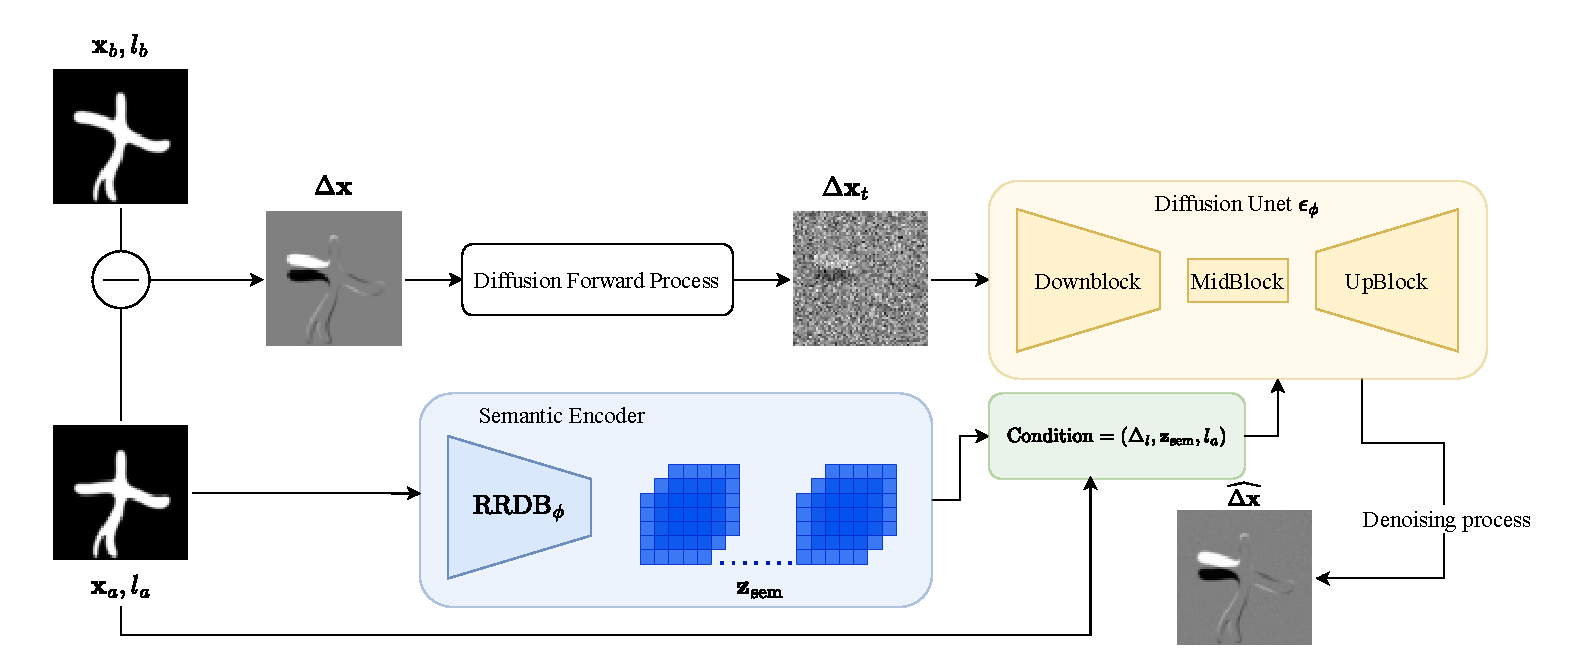
\includegraphics[width=1\linewidth]{figures/model-tdm.pdf}
    \caption[Overview of TDM framework]{Overview of our Temporal Diffusion Model (TDM). Our model takes as input the residual change $\Delta\rvx$ between 2 time points $l_a < l_b$, the conditions to the model are: the current baseline age $l_a$, a list of spatial representations extracted from RRDB \cite{zhang2018RRDB} encoder, the time interval $\Delta_l$. During \textbf{training}, the inputs go through normal diffusion forward-backward process and conditional UNet learns to predict the added noise. At \textbf{inference}, we sample a Gaussian random noise $\rvx_T \sim \mathcal{N}(0, \mathbf{I})$, use trained UNet to denoise with DDIM sampling scheme to predict the residual change. The target image is constructed by adding predicted residual to baseline image $\widehat{\rvx_b} = \rvx_a + \widehat{\Delta\rvx}$}
    \label{fig:model-tdm}
\end{figure}

In this section, we come back to our spatial-temporal setting and introduce our framework to use diffusion model to learn temporal dependencies between samples. As mentioned earlier, one major challenge in unsupervised anomaly detection in MRI scans is the presence of missing scans. Consequently, this raises the important task of imputing missing data based on the available observations. Consequentially, this raises an important domain of imputation of missing data, based on observation. We denote $\mathbf{X}^{\mathcal{O}}_{i} = \{\rvx_1, \rvx_2, \dots, \rvs_L\}$ as our set of observed data, and $\mathbf{X}^{\mathcal{M}}_{i} = \{\rvx_1, \rvx_2, \dots, \rvs_M\}$ the set of missing data that we want to impute, for a patient $i$. Since both training and inference are performed on a per-patient basis, we drop the subscript $i$ for brevity. Our problem setting for temporal diffusion model becomes to learn the conditional distribution of $p(\rvx_m | \rvx_l)$ with $m \in [1 \dots M]$ and $l \in [1 \dots L]$. Our model operates as an autoregressive model that sequentially reconstructs the follow up sample from the previous one, so we have $m < l$. We note that $m$ and $l$ do not need to be consecutive, so $(l - m) \geq 1$.

% We note that the ideal situation would be to learn the joint distribution of all missing data at once, conditioned on all observed data. 

To characterize temporal features within sequences, we adopt the implementation of Temporal-Aware Diffusion Model (TADM) \cite{litricoTADMTemporallyAwareDiffusion2024}. Compared to other existing SOTA models, TADM offers several advantages: 
\begin{itemize}
    \item It provides more flexibility than approaches based on interpolation (\cite{lozuponeLDAE2025}), which requires two input images to be able to generate (interpolate) missing images in between. On the other hand, TADM has the capacity of generating follow up image in any time point in the future based on current image. 
    \item Instead of learning the whole age-related changes within the image, TADM is trained by learning the residual changes between 2 time points. This reduces the complexity of the problem, and minimize the generation errors. 
    \item Consequently, TADM conditions the model on the age gap between the input and output scans rather than directly on the output age. The authors argue that because the same age gap can happen between scans acquired at difference ages, conditioning on age gap avoids the necessity of including samples from every age group in the training set. This is particularly beneficial when the dataset has limited samples in some age groups \cite{litricoTADMTemporallyAwareDiffusion2024}.
\end{itemize}

By combining age gaps (time interval) and residual changes (spatial difference), TADM is trained to learn the distribution of temporal progression. During training, we use pairs of images denoted as $\rvx_a$ and $\rvx_b$, acquired from the same patient at two different time points $l_a < l_b$. These scans are used to compute the residual change $\Delta\rvx = \rvx_b - \rvx_a$, which represents the image growth over the interval $\Delta_l = l_b - l_a$. TADM takes $\Delta\rvx$ and $\Delta_l$ as input and undergoes the standard forward–backward diffusion process to learn the underlying distribution $p(\Delta\rvx \mid \Delta_l)$. At inference, by performing the denoising process, we can sample $\widehat{\Delta\rvx}$ given a baseline age $l_a$ and time interval $\Delta_l$. The future image at $l_b$ is then predicted as $\widehat{\rvx_b} = \rvx_a + \widehat{\Delta\rvx}$. \cref{fig:model-tdm} shows an overview of our TDM framework. 

One major concern with this approach is that different patients may exhibit different rates of change over the same time interval. To account for this, TDM also employs an encoder to extract a non-spatial representation of the input, which is then used as a conditional signal to guide the diffusion process. We make the underlying assumption that the current image contains the most meaningful information about a patient’s state up to this point. In other words, the sequence of images can be viewed as a Markov chain, where future images depend only on the previous one. In addition, we also condition the diffusion process on baseline age $l_a$, under the assumption that the rate of change varies across different ages. Following \cite{litricoTADMTemporallyAwareDiffusion2024}, our TDM comprises two blocks: i) an encoder to extract semantic representation of baseline image, and ii) an UNet block as diffusion model to predict the noises added. Our TDM differs from TADM in that TADM employs an additional Brain Age Estimation (BAE) module to predict the age gap between the predicted image $\widehat{\rvx_b}$ and the baseline $\rvx_a$. It then incorporates the difference between the predicted age gap, $\widehat{\Delta_l} = BAE(\widehat{\rvx_b}, \rvx_a)$, and the true age gap $\Delta_l$ into its loss function. Conceptually, this can be interpreted as an adversarial loss, similar to that used in \ac{GAN} models. This requires additional step of pretraining the BAE module, and we omit it in our experiment for simplicity. Our denoising U-Net is also a conditional diffusion model that follows the same methodology as SDM. For the semantic encoder, we employ the Residual-in-Residual Dense Blocks (RRDB) module \cite{zhang2018RRDB}. Unlike the semantic encoder in SDM (ResNet50), RRDB outputs a list of spatial representations of the input, denoted as $\rvz_{\text{sem}, i} \in \mathbb{R}^{h \times w}$, corresponding to the $i$-th block of the RRDB.
\begin{description}
    \item[Training]: during diffusion step, TDM is trained to predict the noise $\epsilon$ added to the input $\Delta_l$ at time step $t$. The loss function from \cref{eq:loss-ddpm} is updated to incorporate patient specific data as follows: 
    \begin{equation}
    \label{eq:loss-tdm}
        \begin{aligned}
        \mathcal{L} (\theta, \omega) &= ||\epsilon - \epsilon_{\theta} (\Delta\rvx_t, t; \Delta_l, l_a, \mathbf{Z}_a ||^2 \\
        \mathbf{Z}_a &= \mathrm{Enc_{\omega}}(\rvx_a))
        \end{aligned}
    \end{equation}
    where $\Delta\rvx_t = \sqrt{\bar\alpha} \Delta\rvx_0 + \sqrt{\bar\alpha_t} \epsilon$ (\cref{eq:xt-from-x0}), $t \sim \mathrm{Unif}[1, T]$ is the time step, $z_a$ is latent representation of baseline image from RRDB encoder. Similar to our spatial diffusion model, parameters of UNet and Encoder, $\theta$ and $\omega$ respectively, are jointly trained through backpropagation. 
    
    \item[Inference]: our model impute missing scans by an autoregressive process. Given a sequence of observed data $\mathbf{X}^{\mathcal{O}}_{i} = \{\rvx_1, \rvx_2, \dots, \rvs_L\}$, we impute the missing image at time $m$ by finding the closest image from the observed set $\rvx_l \in \mathbf{X}^{\mathcal{O}}$ such that $l < m$. Our model takes as inputs baseline image $\rvx_a$ and time interval with respect to baseline time $\Delta_l = m -l$. The reverse process starts from random Gaussian noise $\Delta_T \sim \mathcal{N}(0; \mathbf{I})$ and progressively denoises through $\epsilon_{\theta}(\Delta_T, t; \rvx_a, \Delta_l, z_a)$. The predicted residual change $\widehat{\Delta_l}$ is then added to baseline image to generate missing image $\widehat{\rvx_m} = \rvx_a + \widehat{\Delta_l}$. 
\end{description}

\section{TDM implementation}
\label{sec:tdm-implement}

\paragraph{UNet}: Our temporal diffusion model is modified from TADM implementation \cite{litricoTADMTemporallyAwareDiffusion2024} \footnote{Available at \href{https://github.com/MattiaLitrico/TADM-Temporally-Aware-Diffusion-Model-for-Neurodegenerative-Progression-on-Brain-MRI}{https://github.com/MattiaLitrico/TADM-Temporally-Aware-Diffusion-Model-for-Neurodegenerative-Progression-on-Brain-MRI}}. Similar to base diffusion model, our UNet comprises input blocks (with downsampling layer), a middle block, and out blocks (with upsampling layer) which are the symmetric counterparts of corresponding downsampling blocks. Down and Up blocks contain 4 levels with channel multipliers of $[32, 64, 128, 256]$. Unlike SDM model, each level in TDM has 2 residual blocks (ResBlock), followed by downsampling (upsampling) block. We omit cross-attention layers in the TDM, as the model operates on residual changes $\Delta \rvx$ rather than the original image $\rvx$, where spatial information is less prominent. This is similar to the implementation from TADM paper. 
\paragraph{Condition signals}: similar to SDM, time step condition $t$ is embedded using sinusoidal embeddings. The condition dimension is $d_{cond} = 32$. For semantic encoder, we use RRDB \cite{zhang2018RRDB} as our backbone network, with 8 blocks and each block has 64 channels. The RRDB is not initialized but is trained from scratch jointly with UNet module. Other patient-specific data, such as age $l_a$ and age difference $\Delta l$, are projected using a linear layer to match the dimension of the time embedding vector. Unlike the SDM, all conditions are injected into the ResBlocks by being summarized with the model’s hidden state. We note that all conditions (except semantic encoded $z_a$) are represented as vectors, while the hidden states are spatial representations produced by Conv2D layers. Therefore, the summation is performed via broadcasting. Formally we have $h := h + \psi_1(t) + \psi_2(l_a) + \psi_3(\Delta_l) + z_{a}$, with $\psi_1, \psi_2, \psi_3$ are trainable projection layers applied to time step, age and time interval, respectively. 
\paragraph{Training configuration}: TDM is trained with 500 epochs, using Adam optimizer with learning rate $2.5 \times 10^{-4}$. Similar to SDM, we employ EMA strategy to smooth out parameters, with EMA decay rate is $0.9999$ and EMA is updated after every 10 batches. \cref{tab:tdm-config} shows the details configurations of our TDM network.

\begin{table}[h]
\captionsetup{justification=raggedright,singlelinecheck=false}
\caption{Temporal Diffusion Model (TDM): configurations and parameters}
% \resizebox{\columnwidth}{!}{%
\begin{tabular}{ll}
\toprule
\multicolumn{2}{l}{\textbf{Encoder $\mathrm{Enc}_{\omega}$}} \\
\midrule
Backbone & \texttt{RRDB} \cite{zhang2018RRDB} \\
Input Modality & $1 \times 64 \times 64 $ \\
RRDB number of blocks & 8 \\
RRDB number of features & 64 \\
\midrule
\multicolumn{2}{l}{\textbf{Diffusion UNet $\epsilon_{\theta}$}} \\
\midrule
Input Shape & $(B, 1, 64, 64)$, with batch size first \\
Channels multipliers & [32, 64, 128, 256] \\
Residual Blocks per Level & 2 \\
Conditional injection & Summarize \\
Dropout & 0.1 \\
Time embedded dimension & $d_{cond} = 32$ \\
Timestep & 1000 \\
Beta Schedule & Linear, $\beta_t \in [10^{-4}, 2 \times 10^{-2}]$ \\
\midrule
\multicolumn{2}{l}{\textbf{Training Configuration}} \\
\midrule
Optimizer & Adam \\
Learning Rate & $2.5 \times 10^{-4}$ \\
EMA Decay & 0.999 \\
Train Batch Size (effective) & 20 \\
Training Duration & 500 epochs / $\sim$4.5 hours \\
Hardware & 1 x Nvidia L40S (45 GiB) \\
\bottomrule
\end{tabular}
% }
\label{tab:tdm-config}
\end{table}

\section{Results}
\label{sec:result-tdm}

In this section, we present our results on using a temporal diffusion model to impute missing data. We demonstrate how the model leverages temporal information from previous observations to generate accurate predictions for the missing values, and we analyze its performance across different scenarios.

% \subsubsection{Imputing missing data}
% \label{sec:result-tdm-recon-error}

\subsection{Imputing subsequence images}
First, we test the reconstruction performance of \ac{TDM} in case of predicting images using information from preceding images. In this simple case, the time interval is $\Delta_l \sim 1$. \cref{tab:tadm-error-previous} shows the similarity metrics and residual errors of subsequently imputation for different anomaly types. We see that \ac{TDM} achieves the best performance on the \texttt{healthy} dataset, which is expected since, during training, our model only sees normal samples. When \ac{TDM} encounters anomalous images during inference, even though semantic representations are provided by the RRDB semantic encoder, our model does not know how to process this information and fails to predict how the anomaly will progress over time. Not only that, but the presence of an anomaly distorts the normal semantic representation, causing our model to produce lower-quality follow-up images. This can be observed in \cref{fig:tadm-impute-gcircle}. Starting from the 2\textsuperscript{nd} observation (5\textsuperscript{th} time point), the anomaly is present, causing subsequent imputations to deteriorate in quality. The anomaly does not grow but rather remains blurry in the following time points.

For healthy dataset, we see that \ac{TDM} achieves very high results, both in terms of similarity metrics and residual errors, with MSSIM closed to 100\%, and LPIPS is around $26 \times 10^{-3}$. 

\begin{table}[htbp]
    \centering
    \begin{adjustbox}{max width=\textwidth}
    \begin{tabular}{lrrrrrr}
    \toprule
    & \multicolumn{4}{c}{Similarity metrics} & \multicolumn{2}{c}{Residual errors} \\
    \cmidrule(lr){2-5} \cmidrule(lr){6-7}
    & SSIM \textuparrow & MSSIM \textuparrow & PSNR \textuparrow & LPIPS (e-3) \textdownarrow & $l1$-error(e-3) \textdownarrow & $l2$-error(e-3) \textdownarrow \\
    \midrule
    \texttt{healthy} & 77.26 & 99.17 & 37.40 & 26.61 & 9.90 & 0.19 \\
    \texttt{growing\_circle} & 75.02 & 97.72 & 23.97 & 33.70 & 17.77 & 6.31 \\
    \texttt{darker\_circle} & 76.68 & 99.07 & 33.05 & 29.19 & 10.99 & 0.52 \\
    \texttt{darker\_line} & 75.82 & 98.90 & 31.73 & 29.31 & 11.60 & 0.71 \\
    \bottomrule
    \end{tabular}
    \end{adjustbox}
    \caption[TDM imputation error - use previous image]{Imputation error: using the previous image to predict the next consecutive image. Results are reported for each type of anomaly.}
    \label{tab:tadm-error-previous}
\end{table}

\subsection{Imputation with random time interval}

\begin{figure}[htbp]
    \centering
    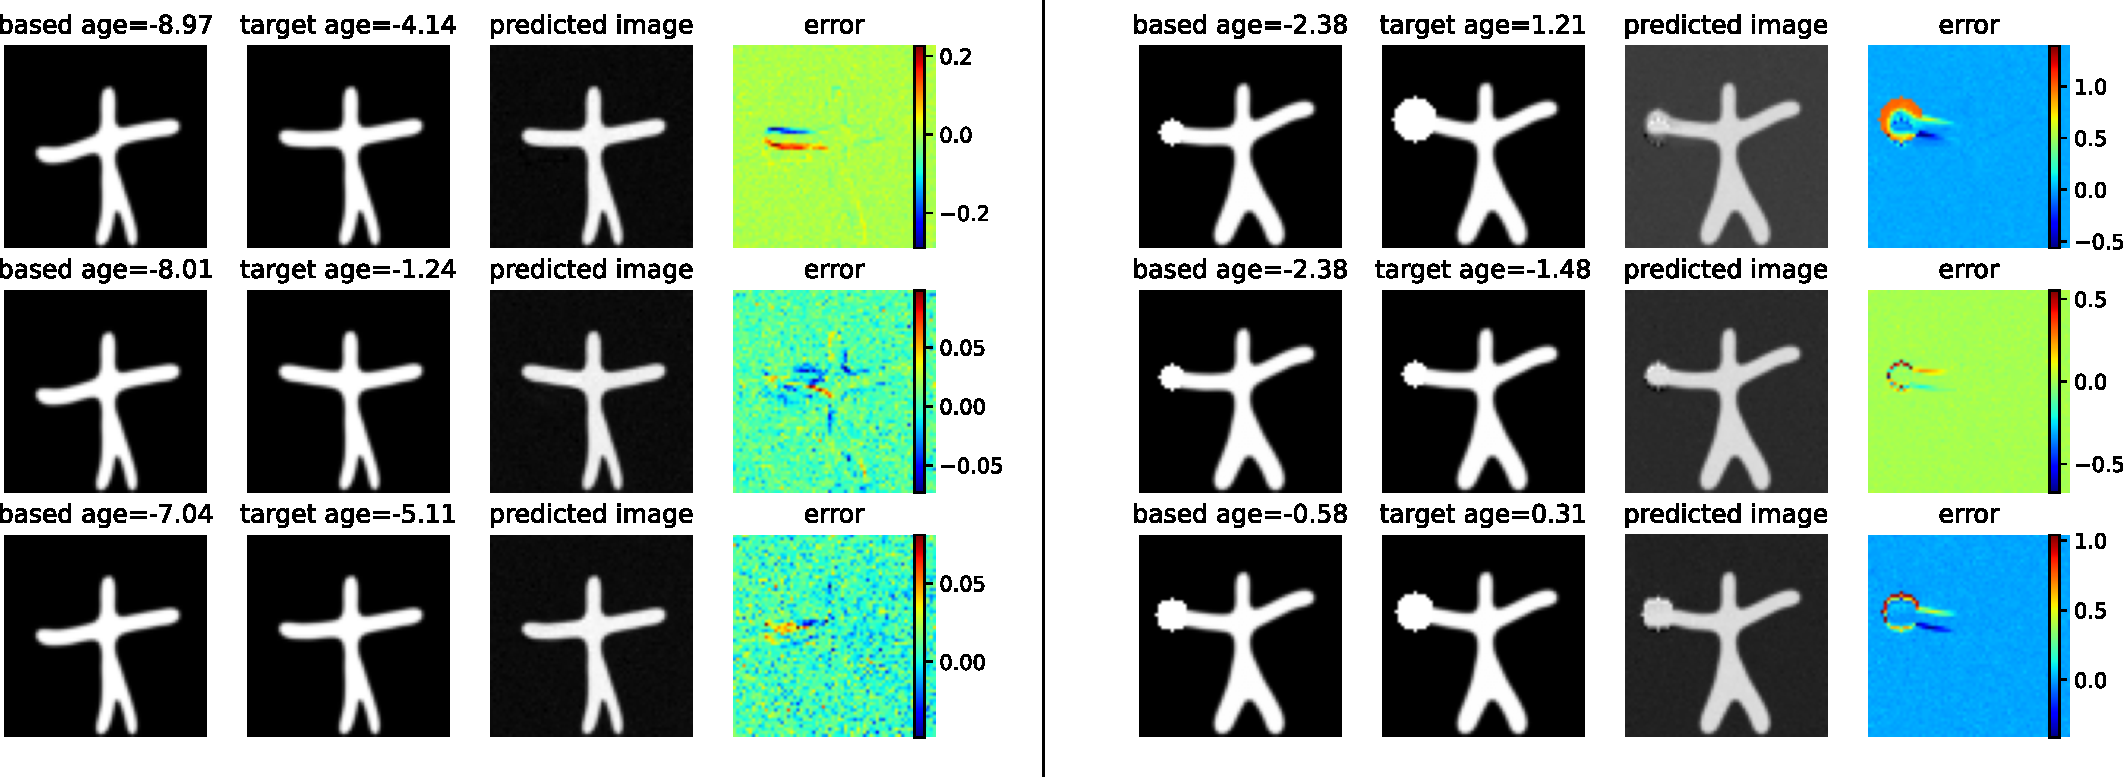
\includegraphics[width=0.8\linewidth]{figures/tadm-randompair.pdf}
    \caption[Example of imputation from TDM - random time interval]{Example of imputation with random time interval. Left: healthy sample. Right: anomaly sample. For each image, from left to right: current image, future image, predicted image, and residual error ($l1$-error)}
    \label{fig:tadm-randompair}
\end{figure}

Next, we test the model capacity of generating follow-up data at arbitrarily $\Delta_l$ time steps in the future. \cref{tab:tadm-error-randompair} reports reconstruction errors for healthy dataset. Results are reported as average of different time gap group. Gap bin $(0-1)$ corresponds to our previous case: imputing subsequence data. We clearly see that the quality decreases as time gap increases, for both similarity metrics and pixel residual errors. The only exception is LPIPS metrics, where we see the best result is obtained at time point really far into the future (time gap bin $(10-11)$), although the differences is small compared to case of subsequent imputation. 

This result can be explained by the fact that the residual growth between 2 consecutive time points is relatively smaller. So even though our model is trained with all random pairs of images (thus it is trained with all time differences), its performance is best when we use preceding image as input conditions. \cref{fig:tadm-randompair} shows examples of generating follow-up images with different time gap. 

\begin{table}[htbp]
    \centering
    \begin{adjustbox}{max width=\textwidth}
    \begin{tabular}{lrrrrrr}
    \toprule
    & \multicolumn{4}{c}{Similarity metrics} & \multicolumn{2}{c}{Residual errors} \\
    \cmidrule(lr){2-5} \cmidrule(lr){6-7}
    $\Delta_l$ gap group & SSIM \textuparrow & MSSIM \textuparrow & PSNR \textuparrow & LPIPS (e-3) \textdownarrow & $l1$-error(e-3) \textdownarrow & $l2$-error(e-3) \textdownarrow \\
    \midrule
    0-1 & \textbf{84.882} & \textbf{99.158} & \textbf{38.266} & 25.867 & \textbf{9.001} & \textbf{0.151} \\
    1-2 & 83.955 & 99.118 & 36.778 & 26.513 & 9.769 & 0.226 \\
    2-3 & 83.422 & 99.037 & 34.670 & 28.398 & 10.835 & 0.362 \\
    3-4 & 84.150 & 98.921 & 32.524 & 28.877 & 11.828 & 0.630 \\
    4-5 & 83.235 & 98.826 & 31.843 & 29.618 & 12.453 & 0.774 \\
    5-6 & 82.772 & 98.744 & 30.906 & 31.476 & 13.255 & 0.898 \\
    6-7 & 83.273 & 98.635 & 30.372 & 31.266 & 14.002 & 1.040 \\
    7-8 & 82.625 & 98.532 & 29.580 & 32.333 & 14.432 & 1.215 \\
    8-9 & 83.880 & 98.564 & 29.427 & 29.821 & 14.433 & 1.289 \\
    9-10 & 83.127 & 98.507 & 29.099 & 27.434 & 15.178 & 1.440 \\
    10-11 & 83.329 & 98.473 & 28.870 & \textbf{25.325} & 15.436 & 1.372 \\
    11-12 & 76.029 & 98.373 & 26.884 & 29.327 & 17.134 & 2.078 \\
    \bottomrule
    \end{tabular}
    \end{adjustbox}
    \caption[TDM imputation error - use random time interval]{Imputation errors: using random pairs with different time interval. Results are reported as the average for each time gap group. Best results are highlighted in \textbf{bold}}
    \label{tab:tadm-error-randompair}
\end{table}

% \paragraph{Imputation of sequence}
\cref{fig:tadm-impute-error} shows examples of imputing all missing images based on observed data. TDM generates images in an autoregressive process. Starting from an observed time point, the model predicts the next succeeding image, and this newly generated image becomes the baseline for the following prediction. The process continues until the next observed time point. 

\begin{figure}[htbp]
    \centering
    \begin{subfigure}{0.68\textwidth}
        \centering
        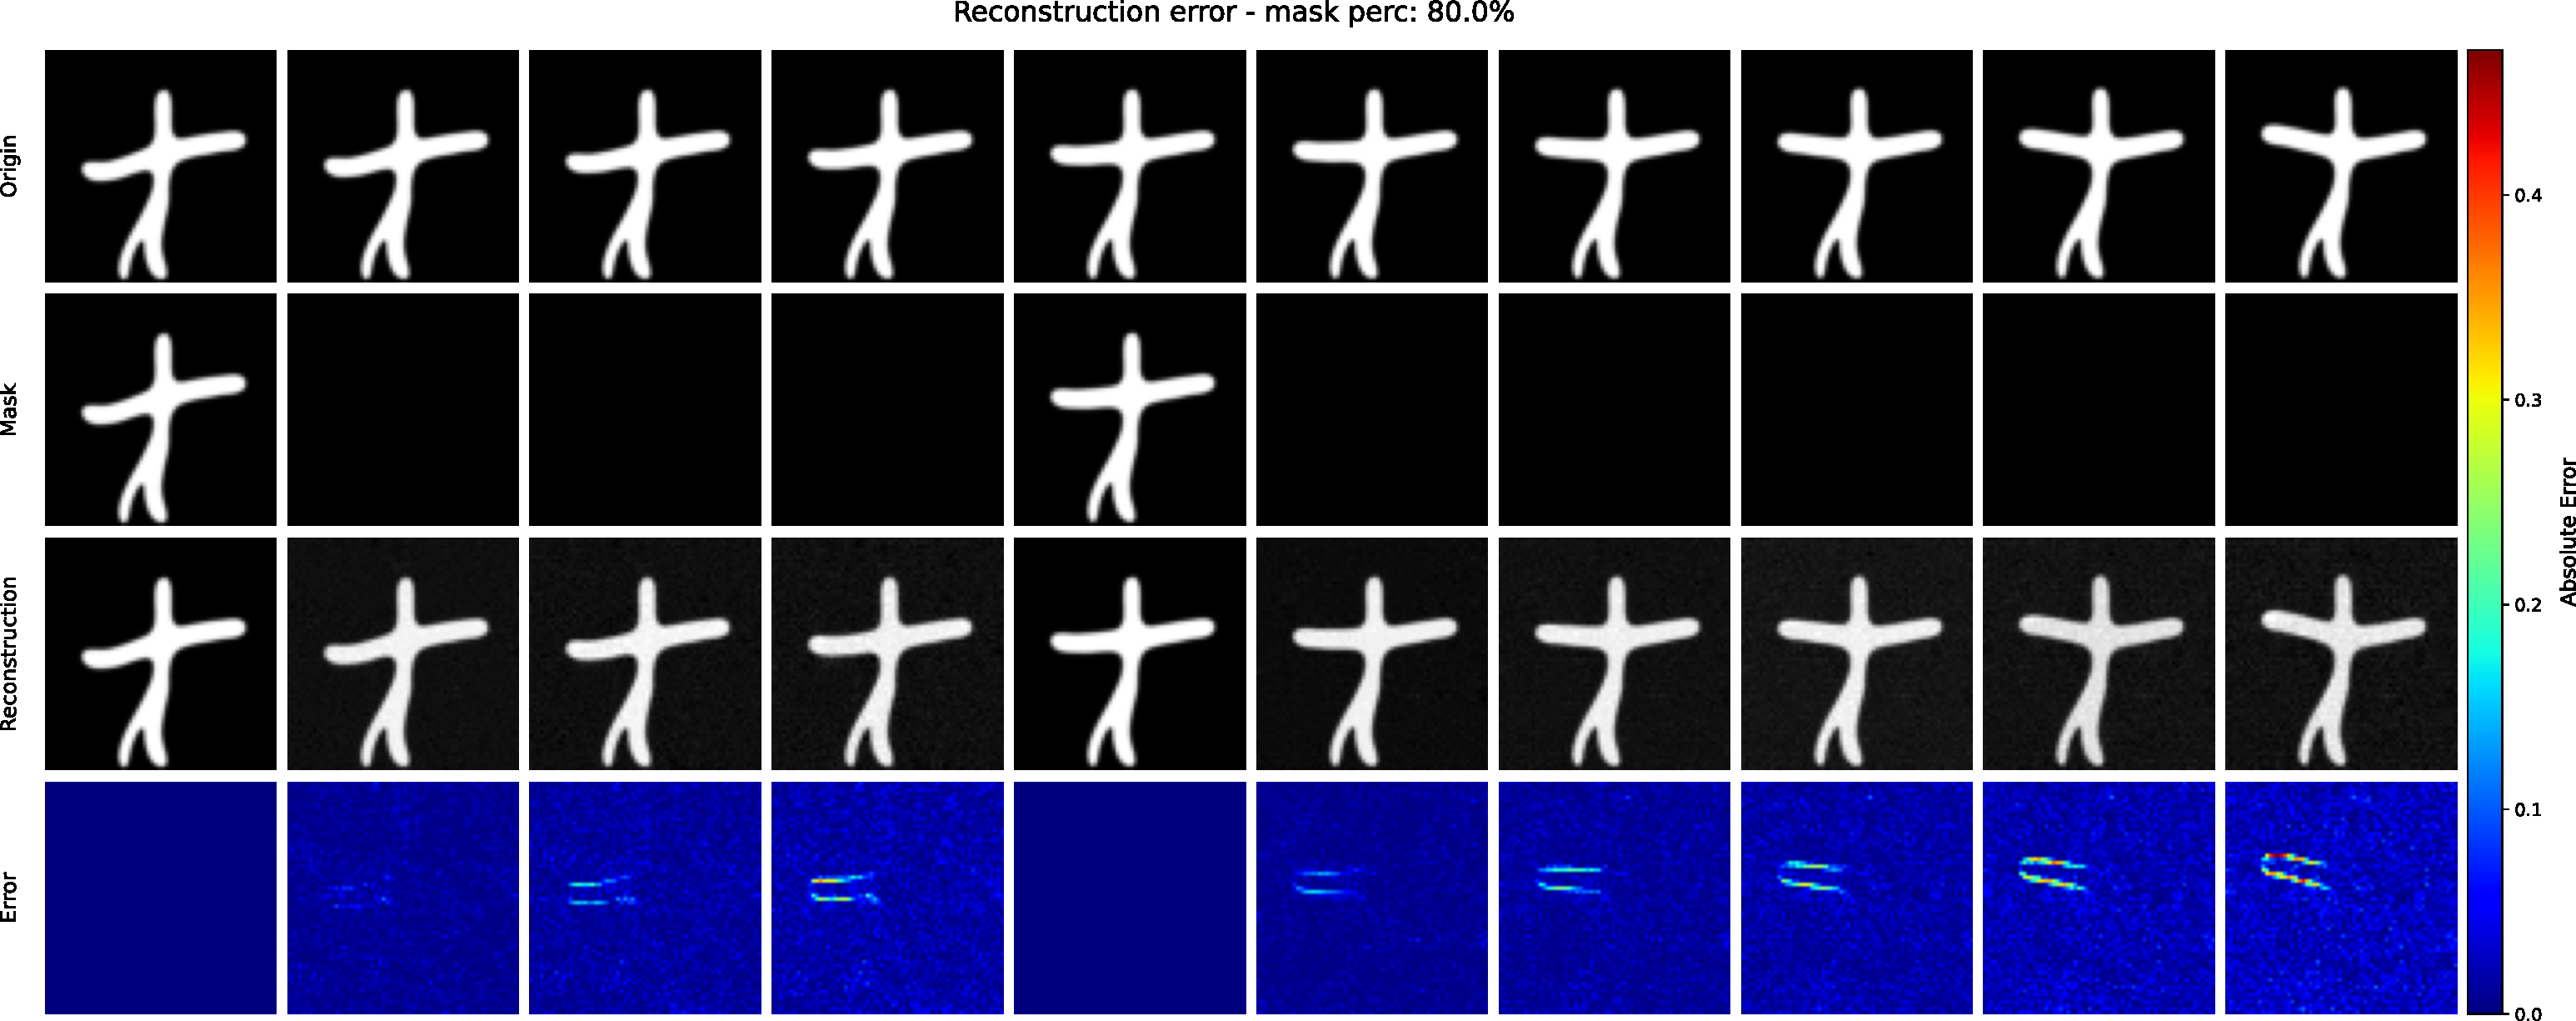
\includegraphics[width=1.0\linewidth]{figures/tadm-impute-healthy.pdf}
        \caption{Imputation for healthy subject.}
        \label{fig:tadm-impute-healthy}
    \end{subfigure}
    \hfill
    \begin{subfigure}{0.68\textwidth}
        \centering
        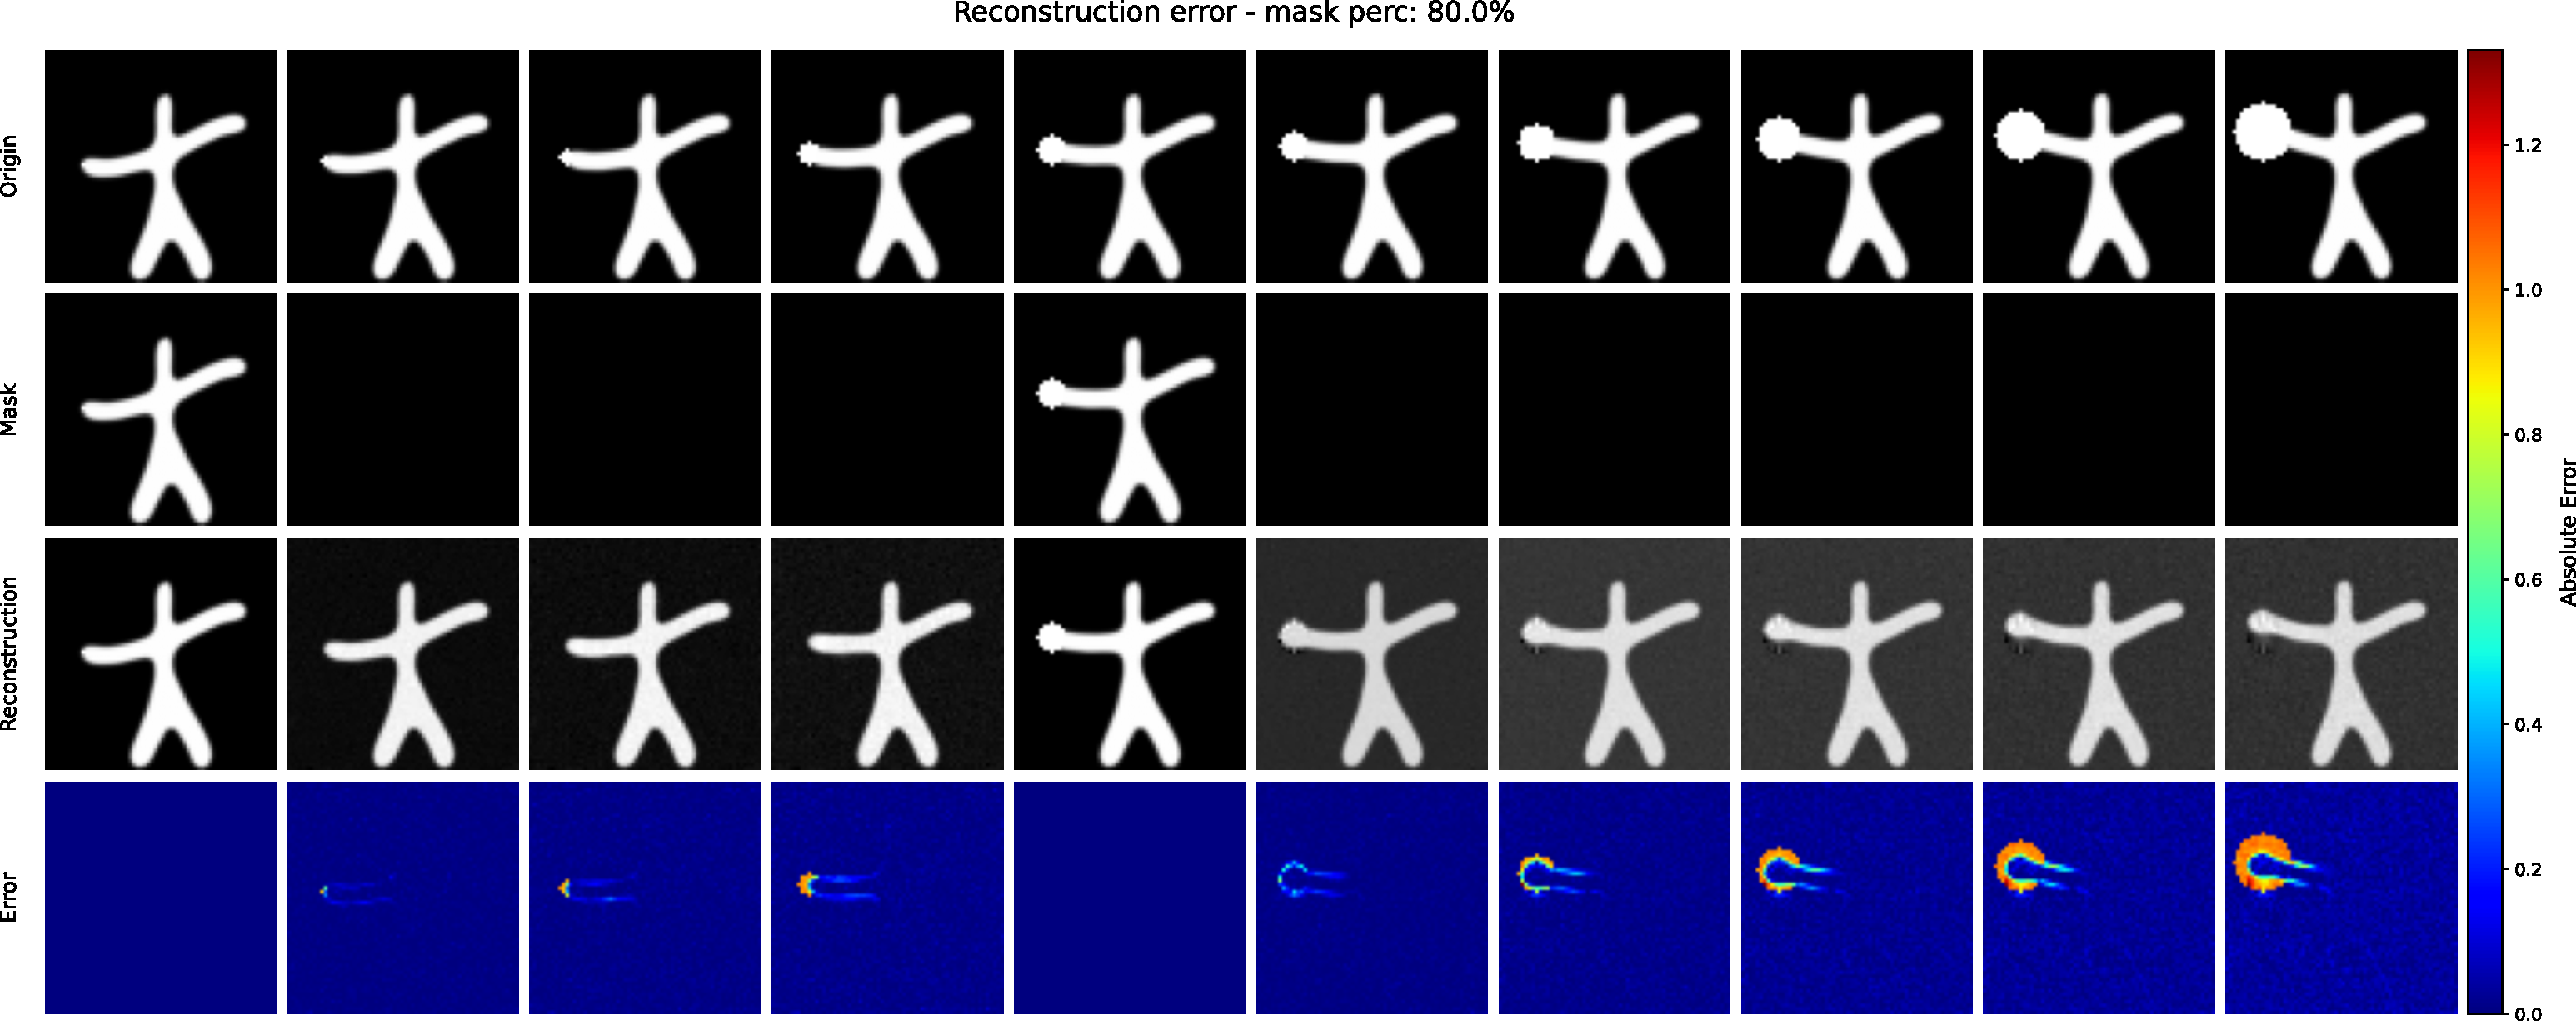
\includegraphics[width=1.0\linewidth]{figures/tadm-impute-gcircle.pdf}
        \caption{Imputation for anomaly subject.}
        \label{fig:tadm-impute-gcircle}
    \end{subfigure}
    \caption[Example imputation of missing data sequences using TDM]{Example of imputing missing data from TADM model. \cref{fig:tadm-impute-healthy} shows example from healthy subject, \cref{fig:tadm-impute-gcircle} shows example for anomaly subject. From top to bottom of each image: original data, masked observed data, imputed data sequence, $l1$-error.}
    \label{fig:tadm-impute-error}
\end{figure}

\subsection{Oversampling}

To test the model capacity to generate new samples that follow the same trajectory of observed data, we oversample by using the last observation as condition and generate a number of follow-up images with time interval $\Delta_l = 1$. \cref{fig:tadm-oversample} shows an example of oversampling for healthy subject. All generated images here are completely new and not included in our dataset. From the residual error (compared to the last observation), we see that our model efficiently learn to recognize the moving part of the sequence (the left hand). For each image in the subsequence, it gradually moves this part higher to align with the subject's trajectory.

\begin{figure}[htbp]
    \centering
    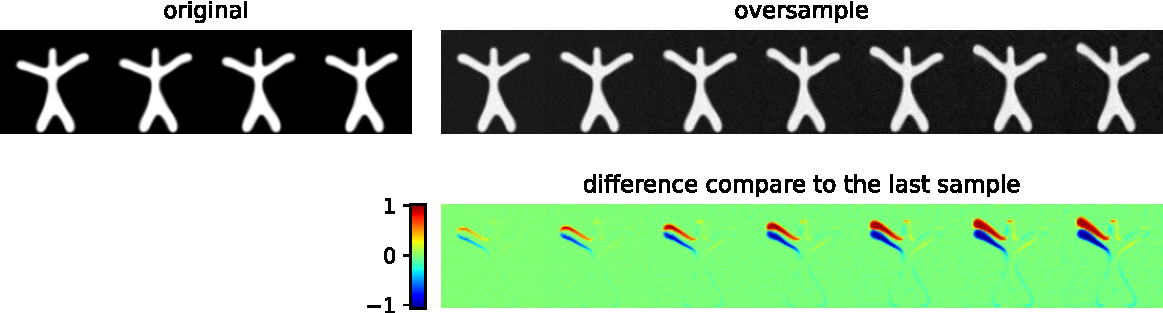
\includegraphics[width=0.75\linewidth]{figures/tadm-oversample.pdf}
    \caption{Example of oversampling with TDM.}
    \label{fig:tadm-oversample}
\end{figure}